%%% Local Variables:
%%% TeX-master: "poster"
%%% End:

\begin{minipage}[t]{0.5\linewidth}
  \begin{center}
    {\Large \textbf{Noise Property}}
  \end{center}
\end{minipage}\hfill
\begin{minipage}[t]{0.5\linewidth}
  \begin{center}
    {\Large \textbf{Dynamical Uncertainty}}
  \end{center}
\end{minipage}\hfill

\begin{minipage}[t]{0.47\linewidth}
  \begin{tikzfigure}[Sensor fusion architecture]
    \centering
    \label{fig:fusion_super_sensor}
    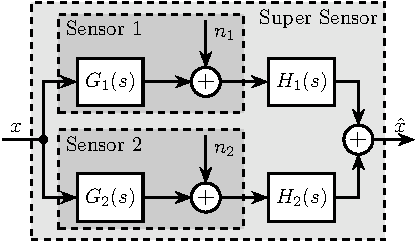
\includegraphics[height=6cm]{figs/fusion_super_sensor.pdf}
  \end{tikzfigure}

  First suppose \textbf{perfectly known sensor dynamics} such that it can be
  inverted:
  \[ G_1(s) = G_2(s) = 1 \]

  The estimate $\hat{x}$ is then:
  \[ \tcmbox{\hat{x} = x + H_1 n_1 + H_2 n_2} \]

  The signal $x$ is kept \textbf{undistorted} while the noises $n_1$ and $n_2$
  are \textbf{filtered out by the complementary filters}.

  \bigskip

  The estimate error $\delta x$ is:
  \[ \delta x \triangleq \hat{x} - x = H_1 n_1 + H_2 n_2 \]

  The PSD of the super sensor \textbf{noise} depends on the \textbf{norm} of the
  complementary filters:
  \[ \tcmbox{\Phi_{\delta x} = \left|H_1\right|^2 \Phi_{n_1} +
      \left|H_2\right|^2 \Phi_{n_2}} \]
\end{minipage}\hfill
\begin{minipage}[t]{0.47\linewidth}
  \begin{tikzfigure}[Fusion of sensors with dynamics uncertainty]
    \centering
    \label{fig:sensor_fusion_dynamic_uncertainty}
    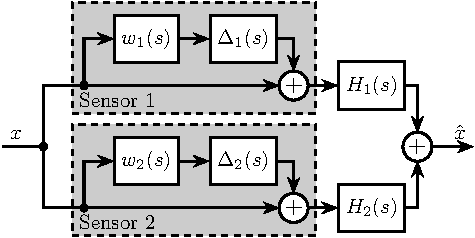
\includegraphics[height=6cm]{figs/sensor_fusion_dynamic_uncertainty.pdf}
  \end{tikzfigure}

  Let's represent sensor dynamic uncertainty by \textbf{multiplicative input uncertainty}:
  \[ \begin{aligned}
      G_i^\prime(s) = G_i(s) [1 + & w_i(s)\Delta_i(s)], \\
      &\forall\Delta_i, \|\Delta_i\|_\infty < 1
    \end{aligned} \]

  The dynamics of the super sensor is:
  \[ \tcmbox{\frac{\hat{x}}{x} = 1 + w_1 H_1 \Delta_1 + w_2 H_2 \Delta_2} \]

  The obtained \textbf{dynamic uncertainty} depends on the \textbf{norm} of the filters (Fig.~\ref{fig:uncertainty_set_super_sensor}).

  \begin{tikzfigure}[Uncertainty set of the super sensor dynamics]
    \label{fig:uncertainty_set_super_sensor}
    \centering
    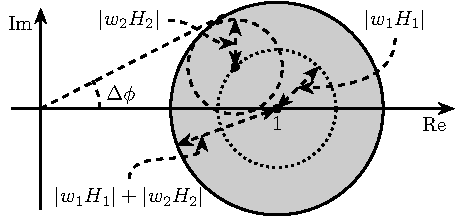
\includegraphics[width=0.8\linewidth]{figs/uncertainty_set_super_sensor.pdf}
  \end{tikzfigure}
\end{minipage}

\bigskip
\sepline
\bigskip

As shown in the analysis above, \textbf{the performance and robustness of the sensor fusion architecture depends on the complementary filters norms}.
Therefore, the development of a synthesis method of complementary filters that allows the shaping of their norm is necessary.